%\documentclass[t]{beamer}
\documentclass[aspectratio=169]{beamer}
\usepackage{helvet}
\usepackage{calc}
\usepackage[utf8]{inputenc}
\usepackage[english]{babel}

\usetheme{Ilmenau}

\setbeamercovered{transparent}
\setbeamertemplate{navigation symbols}{}

\usepackage{units}
\usepackage{amsbsy}
\usepackage{amsmath}
\usepackage{amssymb}
\usepackage{graphics}
\usepackage{graphicx}
\usepackage{epsf}
\usepackage{epsfig}
\usepackage{fixmath}
%\usepackage{pgfmath}
\usepackage{wrapfig}


\title{FOSDEM infrastructure review}
\subtitle{We have become so good, this is basically last year's talk}
\author{Richard Hartmann,\\
RichiH@\{freenode,OFTC,IRCnet\},\\
richih@\{fosdem,debian\}.org}
\date{2019-02-03}


\begin{document}

% hide all subsections
\setcounter{tocdepth}{1}

\begin{frame}
	\titlepage
\end{frame}



%\begin{frame}
%	\frametitle{Statistics}
%	\tableofcontents
%\end{frame}

%\section{asdf}

\begin{frame}
	\frametitle{Repetition}
	\vfill
	\begin{itemize}
		\item This is almost the same talk as last year
		\item Which is good!
		\item One minor thing...
	\end{itemize}
	\vfill
\end{frame}

\begin{frame}
	\frametitle{IPv6 is here}
	\vfill
	\begin{itemize}
		\item First year we had more IPv6-only clients than dual-stack clients
		\item FOSDEM-legacy carries a LOT more VPN traffic
		\item ..so those are probably stuck on v4 for VPN reasons
	\end{itemize}
	\vfill
\end{frame}

\begin{frame}
	\frametitle{Silence before the storm?}
	\vfill
	\begin{itemize}
		\item For the SECOND time in FOSDEM's existence, we have had time to sit down and breathe
		\item Staff was wary about the silence last year, but we kinda felt OK this time
	\end{itemize}
	\vfill
\end{frame}

\begin{frame}
	\frametitle{Word of the conference: "boring"}
	\vfill
	\begin{itemize}
		\item We reached a place of stability
		\item Our changes are now all evolutionary, not revolutionary
		\item Sleep levels are way up, and we like it that way
	\end{itemize}
	\vfill
\end{frame}

\begin{frame}
	\frametitle{Core infra}
	\vfill
	\begin{itemize}
		\item Cisco ASR 1006 for routing, ACLs, NAT64, DHCP
		\item Two servers for all others services, done via Ansible; will get SSDs after this event
		\item All monitoring with Prometheus \& Grafana
		\item Data for public dashboard sent to, persisted with, and served by Cortex on Grafana.com
	\end{itemize}
	\vfill
\end{frame}

\begin{frame}
	\frametitle{Video}
	\vfill
	\begin{itemize}
		\item Capture with our video boxes
		\item Send streams to render farm
		\item Send streams off-site for streaming and cutting into finished videos
		\item Semi-automated review and cutting process via \url{https://github.com/yoe/sreview}
	\end{itemize}
	\vfill
\end{frame}

\begin{frame}
	\frametitle{Render farm}
	\vfill
	\begin{figure}[ht!]
		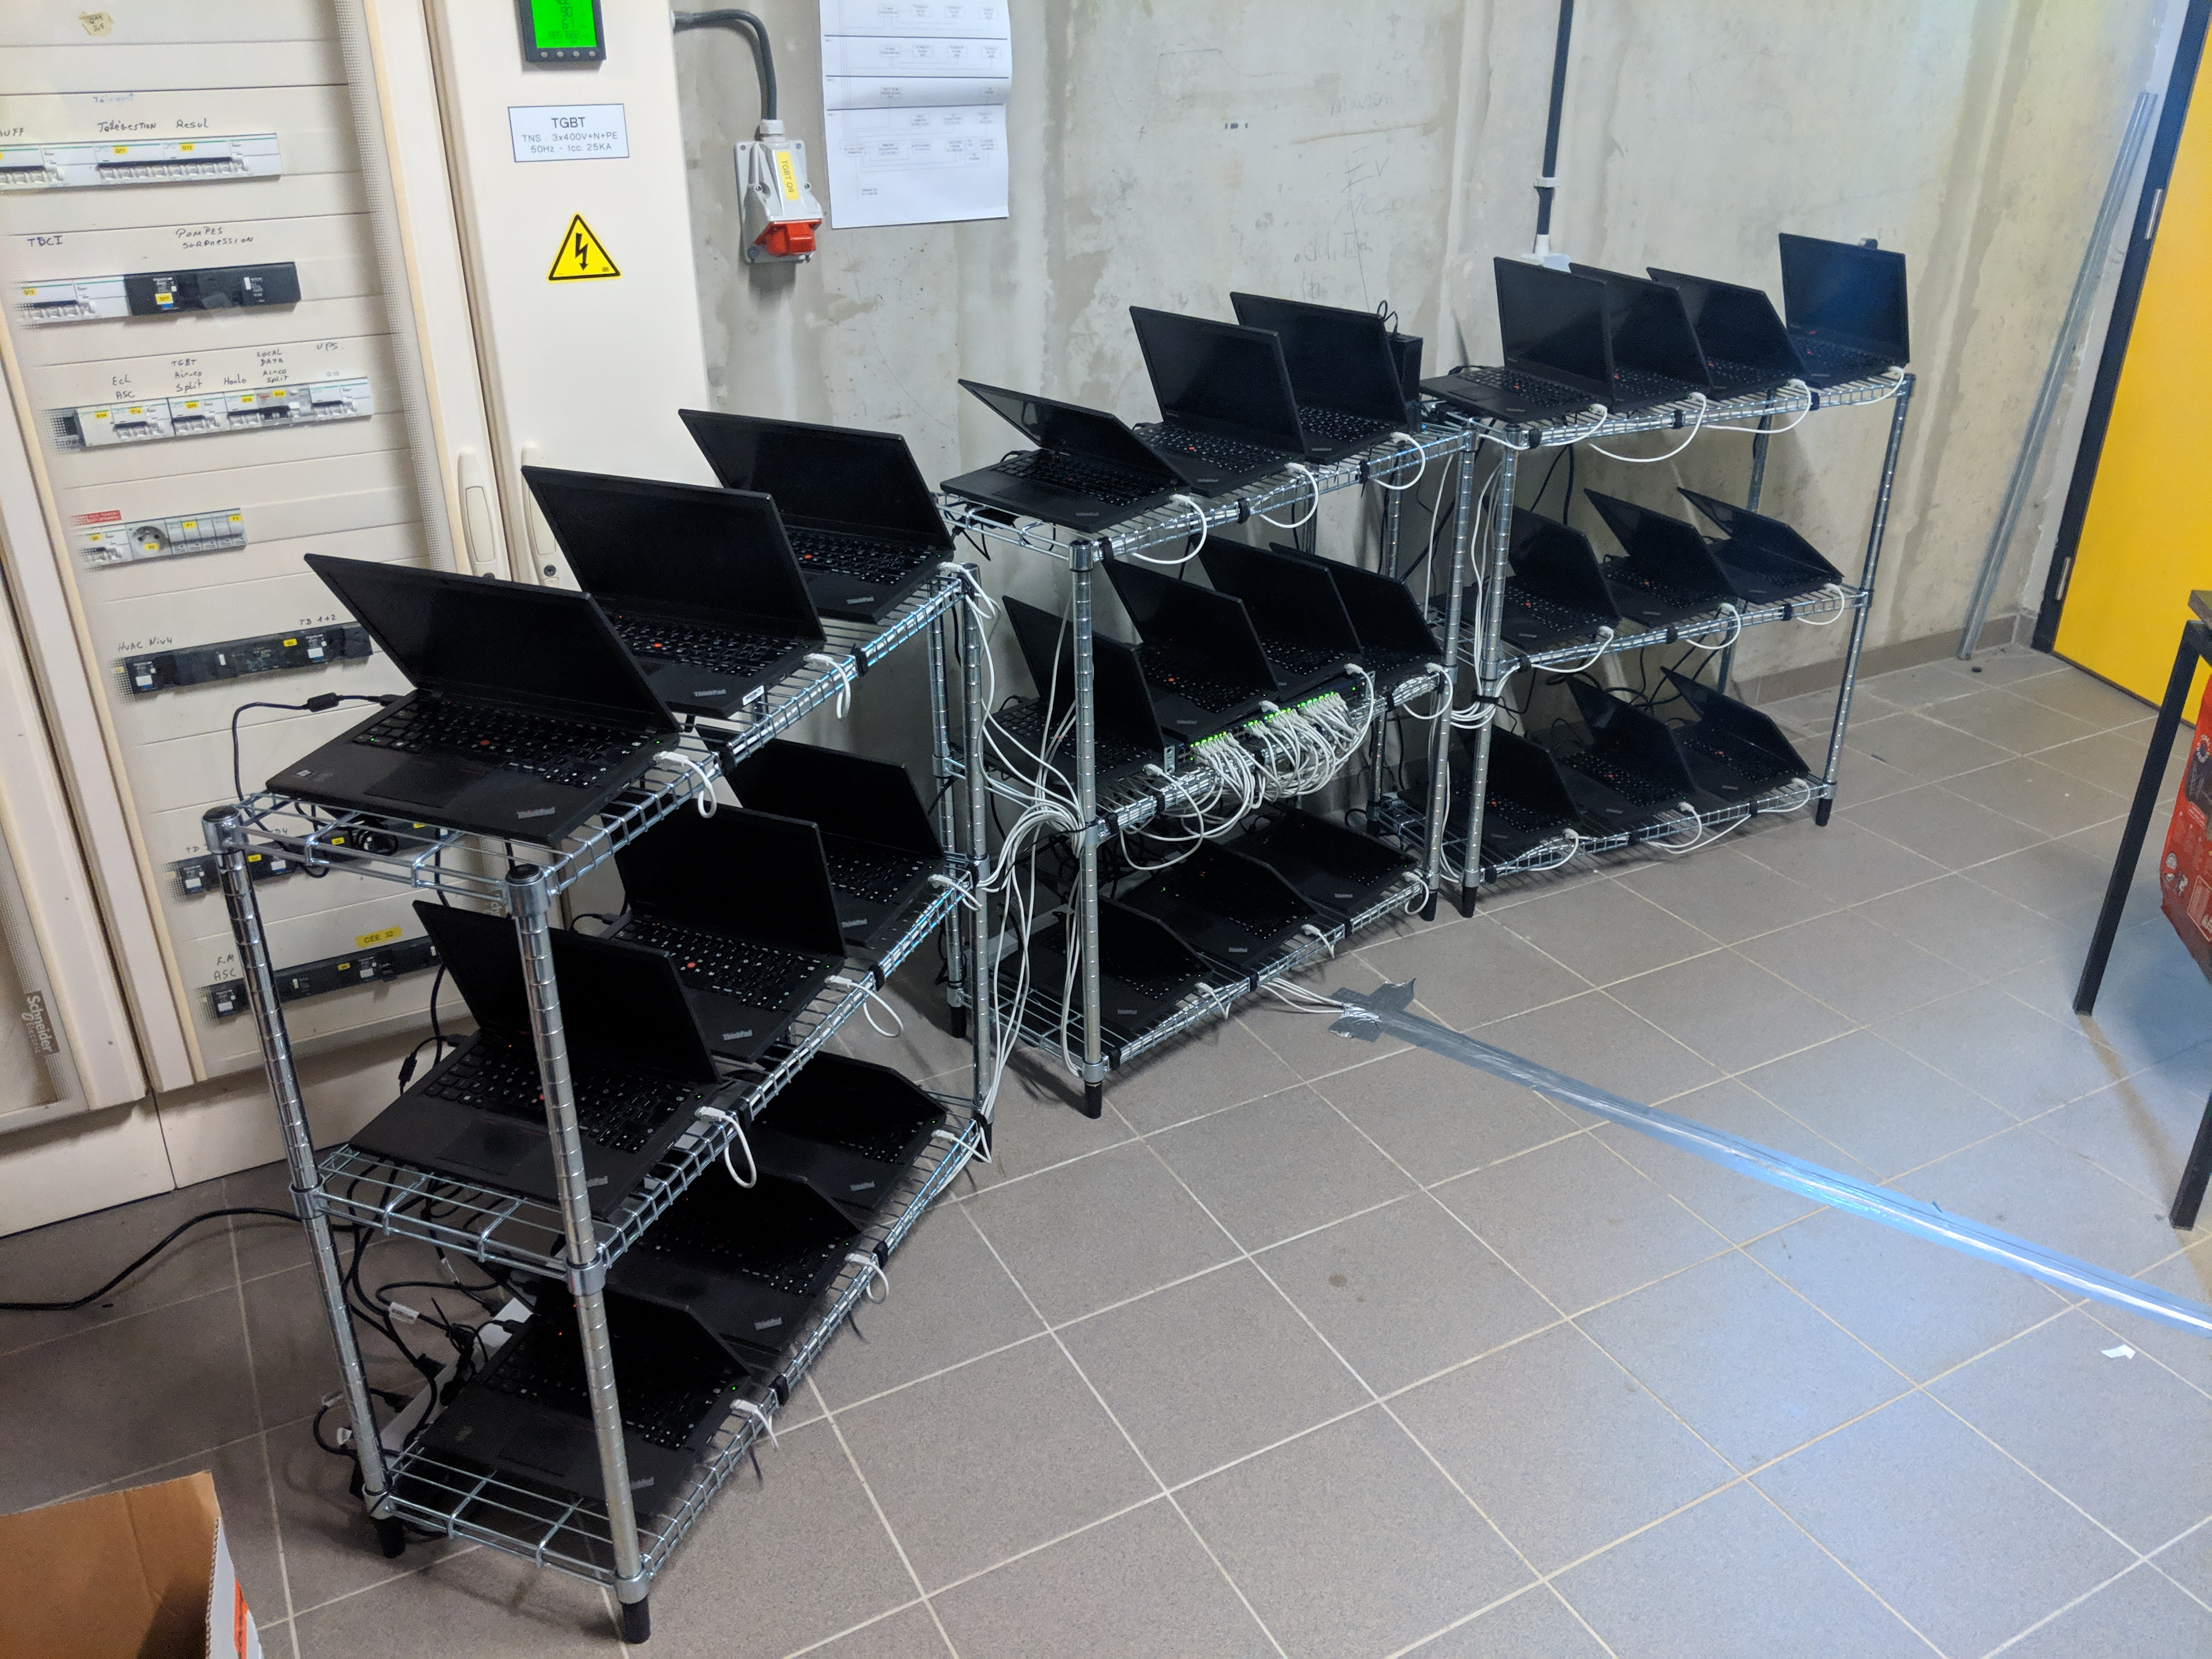
\includegraphics[width=80mm]{render_farm.jpg}
	\end{figure}
	\vfill
\end{frame}

\begin{frame}
	\frametitle{Timelines}
	\vfill
	\begin{itemize}
		\item Installation of router
		\begin{itemize}
			\item 2016: Friday
			\item 2017: December
			\item 2018: December
			\item 2019: December
		\end{itemize}
		\item Network up
		\begin{itemize}
			\item 2015: Saturday 05:00
			\item 2016: Friday 19:00
			\item 2017: Friday 16:00
			\item 2018: Friday 12:00
			\item 2019: Thursday, last hiccups solved on Friday 19:00
		\end{itemize}
	\end{itemize}
	\vfill
\end{frame}

\begin{frame}
	\frametitle{Timelines}
	\begin{itemize}
	\vfill
		\item Monitoring
		\begin{itemize}
			\item 2016: Saturday 12:00
			\item 2017: Saturday 09:00
			\item 2018: January
			\item 2019: January
		\end{itemize}
		\item Video
		\begin{itemize}
			\item 2016: Saturday 11:30
			\item 2017: Saturday 09:30
			\item 2018: Saturday 08:30
			\item 2019: Friday 21:00
		\end{itemize}
	\end{itemize}
	\vfill
\end{frame}


\begin{frame}
	\frametitle{Caveats}
	\vfill
	\begin{itemize}
		\item Know your automation tools
		\item Debugging and fixing is very different from the traditional approaches
		\item The re-use of code and config makes you miss things; but we learned from 2018
		\begin{itemize}
			\item 2018: FOSDEM 2017 background
			\item 2018: Internally, our t-shirt tracker still thought it was 2017
		\end{itemize}
	\end{itemize}
	\vfill
\end{frame}


\begin{frame}
	\frametitle{Only new thing}
	\vfill
	\begin{itemize}
		\item We will be using netbox as our CMDB going forward
		\item Try our monitoring: \\ \url{https://dashboard.fosdem.org}
		\item Clone our conference: \\ \url{https://github.com/FOSDEM/infrastructure}
	\end{itemize}
	\vfill
\end{frame}


\end{document}

%\begin{frame}
%	\frametitle{}
%	\begin{itemize}
%		\item 
%		\item 
%		\item 
%		\item 
%		\item 
%	\end{itemize}
%\end{frame}
